\documentclass[11pt,]{article}
\usepackage[margin=1in]{geometry}
\newcommand*{\authorfont}{\fontfamily{phv}\selectfont}
\usepackage[]{mathpazo}

\usepackage{xcolor}

%TIKZ and Flow chart material
\usepackage{tikz}
\usetikzlibrary{shapes.geometric, arrows}
\tikzstyle{startstop} = [rectangle, rounded corners, minimum width=3cm, minimum height=1cm,text centered, draw=black, fill=red!30]
\tikzstyle{io} = [trapezium, trapezium left angle=70, trapezium right angle=110, minimum width=3cm, minimum height=1cm, text centered, draw=black,fill=white]
\tikzstyle{process} = [rectangle, minimum width=3cm, minimum height=1cm, text centered, draw=black, fill=white]
\tikzstyle{decision} = [diamond, minimum width=3cm, minimum height=1cm, text centered, draw=black, fill=white]
\tikzstyle{smalldecision} = [diamond, minimum width=1cm, minimum height=1cm, text centered, draw=black, fill=white]
\tikzstyle{arrow} = [thick,->,>=stealth]
\tikzstyle{line} = [thick,-]
\tikzstyle{dot} = [circle,inner sep=0.5pt,draw=black, fill=black]


%\tikzstyle{startstop} = [rectangle, rounded corners, minimum width=3cm, minimum height=1cm,text centered, %draw=black, fill=red!30]
%\tikzstyle{io} = [trapezium, trapezium left angle=70, trapezium right angle=110, minimum width=3cm, %minimum height=1cm, text centered, draw=black,fill=white]
%\tikzstyle{process} = [rectangle, minimum width=3cm, minimum height=1cm, text centered, draw=black, %fill=white]
%\tikzstyle{decision} = [diamond, minimum width=3cm, minimum height=1cm, text centered, draw=black, %fill=green!30]
%\tikzstyle{arrow} = [thick,->,>=stealth]




\usepackage{abstract}
\renewcommand{\abstractname}{}    % clear the title
\renewcommand{\absnamepos}{empty} % originally center
\newcommand{\blankline}{\quad\pagebreak[2]}

\providecommand{\tightlist}{%
  \setlength{\itemsep}{0pt}\setlength{\parskip}{0pt}}
\usepackage{longtable,booktabs}

\usepackage{parskip}
\usepackage{titlesec}
\titlespacing\section{0pt}{12pt plus 4pt minus 2pt}{6pt plus 2pt minus 2pt}
\titlespacing\subsection{0pt}{12pt plus 4pt minus 2pt}{6pt plus 2pt minus 2pt}

\titleformat*{\subsubsection}{\normalsize\itshape}

\usepackage{titling}
\setlength{\droptitle}{-.25cm}

%\setlength{\parindent}{0pt}
%\setlength{\parskip}{6pt plus 2pt minus 1pt}
%\setlength{\emergencystretch}{3em}  % prevent overfull lines

\usepackage[T1]{fontenc}
\usepackage[utf8]{inputenc}

\usepackage{fancyhdr}
\pagestyle{fancy}
\usepackage{lastpage}
\renewcommand{\headrulewidth}{0.3pt}
\renewcommand{\footrulewidth}{0.0pt}
%\lhead{\footnotesize Problem Set \#1 }
\lhead{\footnotesize BUEC 311: Problem Set \#1, Thinking like an economist}
\rhead{\footnotesize \today}
\lfoot{\small \copyright }
\cfoot{}
\rfoot{\small \thepage/\pageref*{LastPage}}

\fancypagestyle{firststyle}
{
\renewcommand{\headrulewidth}{0pt}%
   \fancyhf{}
   \fancyfoot[C]{\thepage/\pageref*{LastPage}}
}

%\def\labelitemi{--}
%\usepackage{enumitem}
%\setitemize[0]{leftmargin=25pt}
%\setenumerate[0]{leftmargin=25pt}




\makeatletter
\@ifpackageloaded{hyperref}{}{%
\ifxetex
  \usepackage[setpagesize=false, % page size defined by xetex
              unicode=false, % unicode breaks when used with xetex
              xetex]{hyperref}
\else
  \usepackage[unicode=true]{hyperref}
\fi
}
\@ifpackageloaded{color}{
    \PassOptionsToPackage{usenames,dvipsnames}{color}
}{%
    \usepackage[usenames,dvipsnames]{color}
}
\makeatother
\hypersetup{breaklinks=true,
            bookmarks=true,
            pdfauthor={},
             pdfkeywords = {},
            pdftitle={Problem Set \#1: Thinking like an economist},
            colorlinks=true,
            citecolor=blue,
            urlcolor=blue,
            linkcolor=magenta,
            pdfborder={0 0 0}}
\urlstyle{same}  % don't use monospace font for urls


\setcounter{secnumdepth}{0}


%



\usepackage{setspace}

\title{\vspace{-1.5cm}\Large{BUEC 311: Business Economics, Organization and Management}\medskip\\\Large{Problem Set \#1}
\medskip\\\Large{Thinking like an economist}
}
\date{\vspace{-.75cm}\Large{\today}}

\definecolor{light-gray}{gray}{0.8}


\begin{document}

\vspace{-5cm}\maketitle
 \tikz [remember picture,overlay]
    %\node[yshift=-1.65cm,xshift=0cm] at (current page.north)
    %\node[yshift=-1.65cm,xshift=0cm] at (current page.north)
        %or: (current page.center)
        \node[yshift=-1cm,xshift=6.5cm] at (current page.north west)
        %{
\includegraphics[width=3in]{UA-ASB-COLOUR.png}};
        {
\includegraphics[width=.5\paperwidth]{../images/UA-ASB-COLOUR.png}};
\vspace{-.75cm}		
		\thispagestyle{firststyle}



This week's problems are meant to get you thinking about economics in
everyday life, and exploring some of the topics and vocabulary we've
addressed in the introductory classes.

\begin{enumerate}
\def\labelenumi{\arabic{enumi}.}
\item
  Consider all of the course outlines for the classes you're taking this
  term including mine. You can also use examples from previous courses
  if you choose to do so.

  \begin{enumerate}
  \def\labelenumii{\alph{enumii})}
  \item
    Find one example of a professor using incentive response to drive
    behaviour in the design of their course.
  \item
    Find an example (if you can) of what economists would call a
    perverse incentive, or a rule that likely leads to behaviours that
    the professor might prefer to avoid.
  \item
    Consider some of the decisions you've made this Fall to prepare for
    classes. Which decisions would have changed, and how, if you'd had
    access to an extra \$500? How would you have had to change your
    decisions if you received an unexpected bill for \$500?
  \end{enumerate}
\item
  Think of an example in your life in which you behave as though you
  were following a demand curve (i.e.~when prices of good X drop, you
  buy more).
\end{enumerate}

\centering

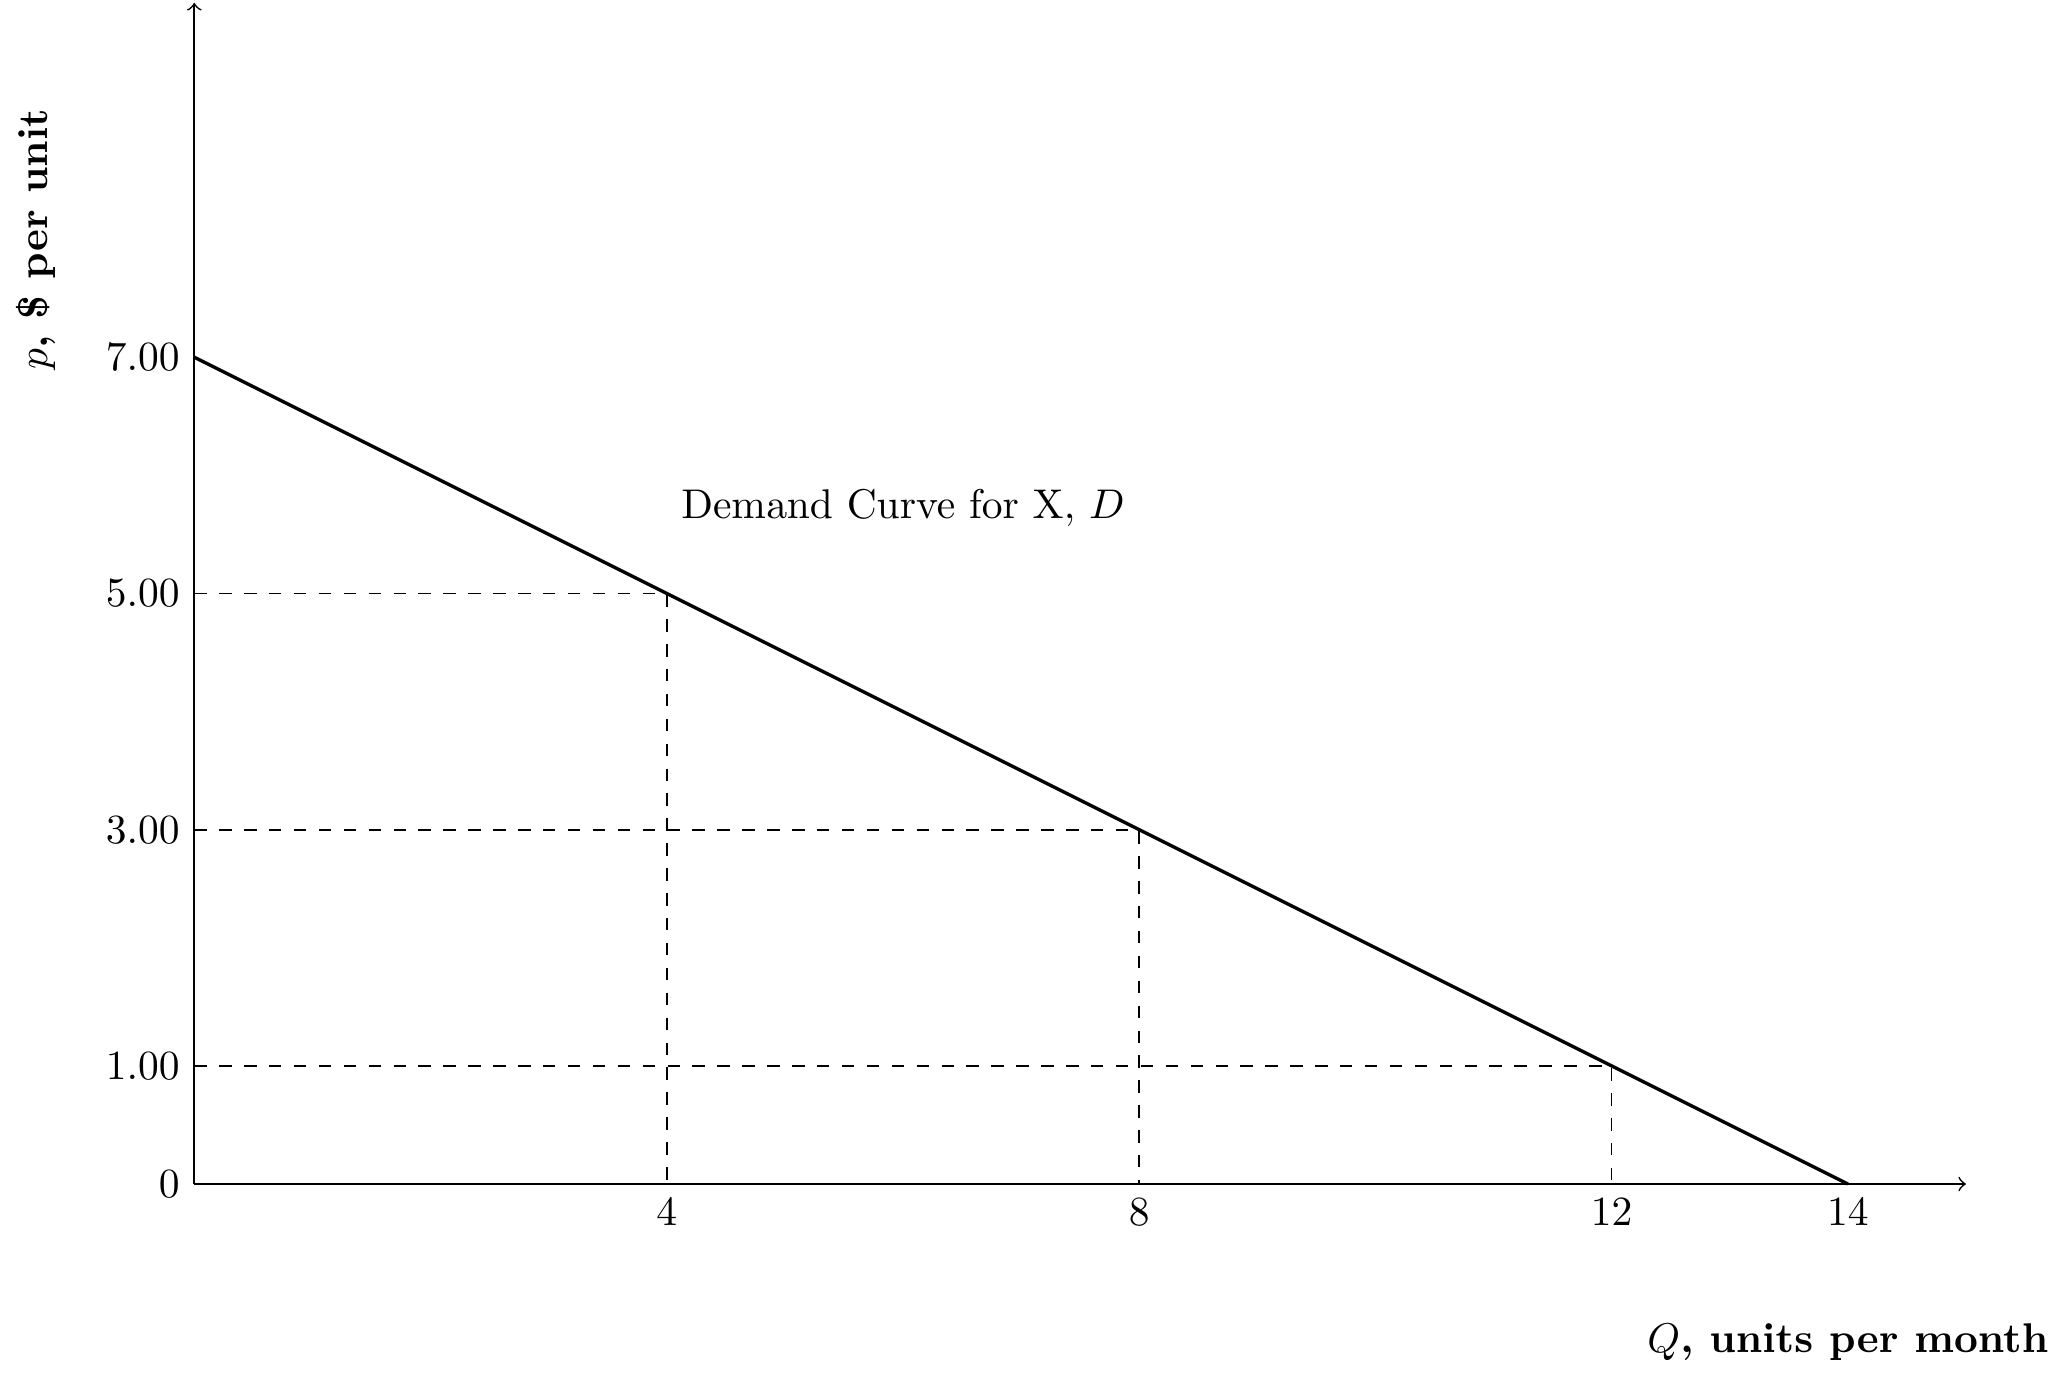
\includegraphics[width=0.65\textwidth]{week_1_problems_files/figure-latex/demand_1-1.png}

\begin{enumerate}
\def\labelenumi{\arabic{enumi}.}
\setcounter{enumi}{2}
\tightlist
\item
  Now, consider the opposite. Think of an example in your life in which
  your consumption of a product or service doesn't appear to be related
  to its price or to your income.
\end{enumerate}

\newpage

\begin{enumerate}
\def\labelenumi{\arabic{enumi}.}
\setcounter{enumi}{3}
\tightlist
\item
  Now, let's switch to the supply side. Can you think of a market or
  firm where you readily see a supply curve functioning like it does in
  an economics textbook?
\end{enumerate}

\centering

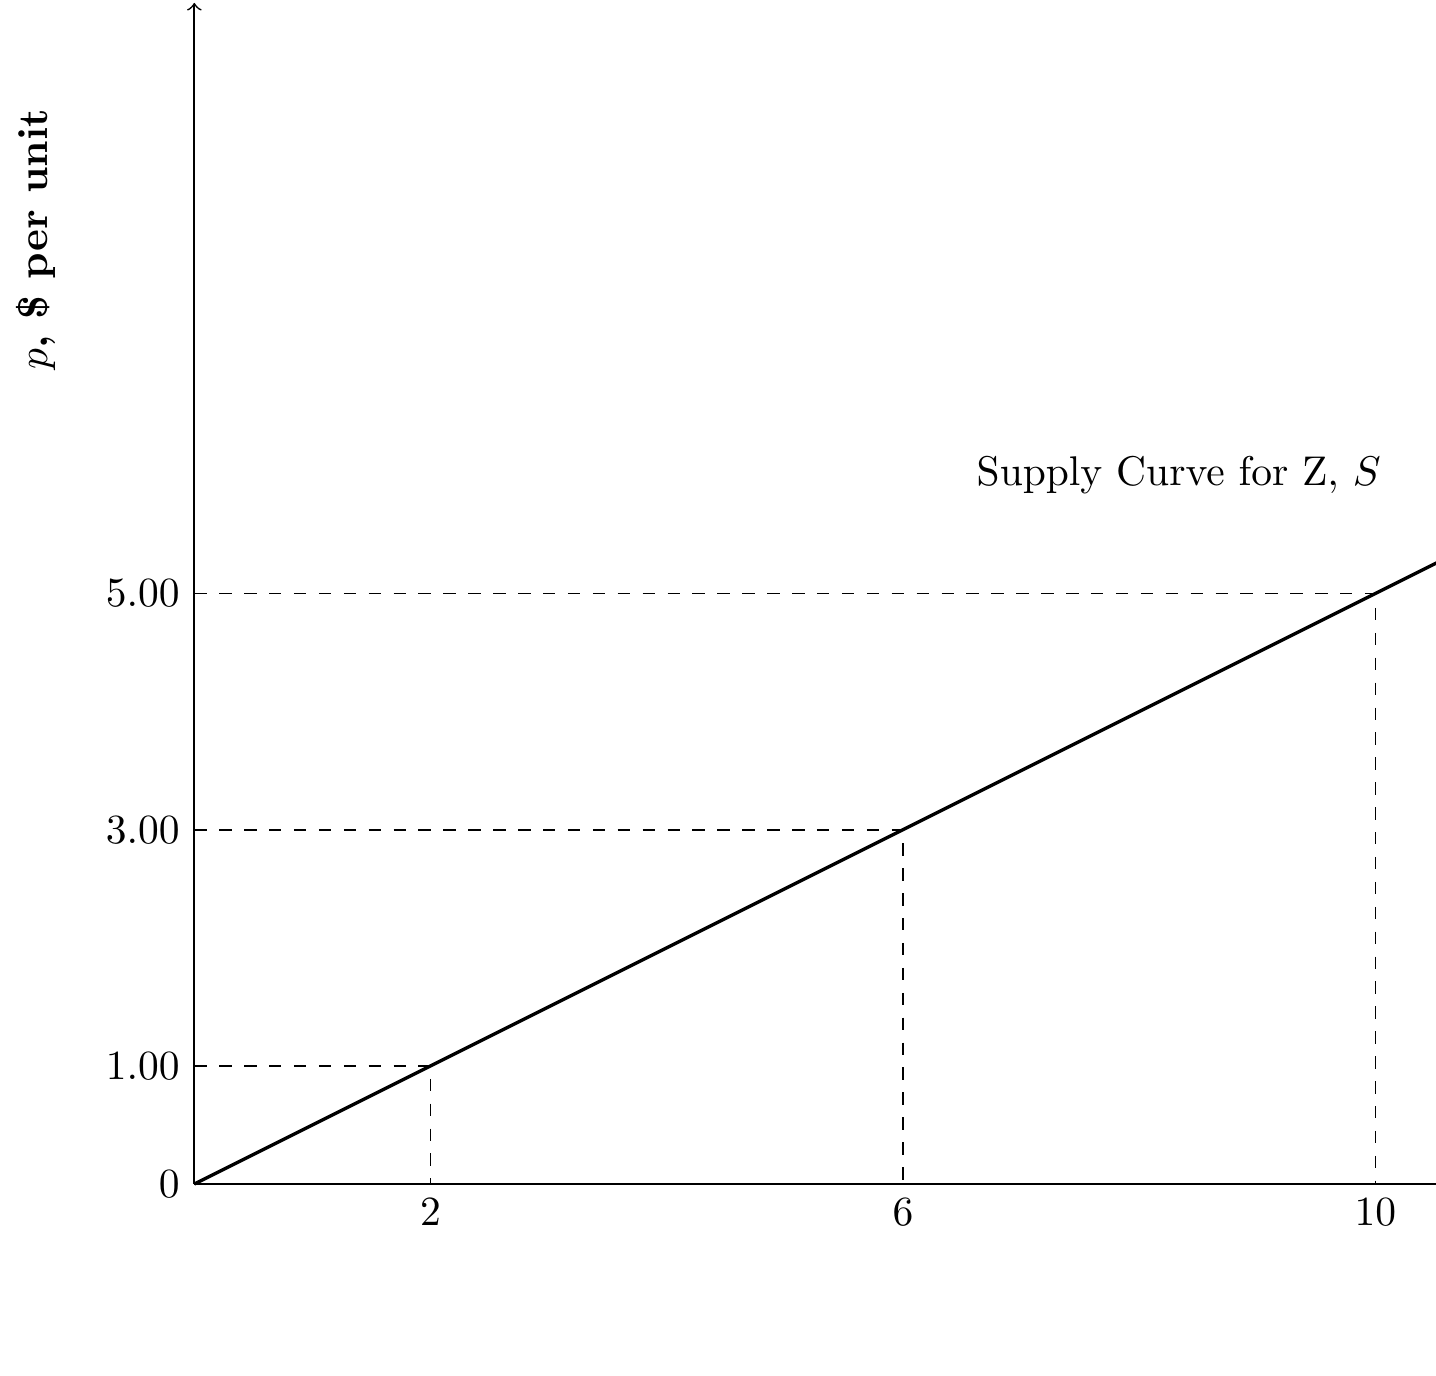
\includegraphics[width=0.5\textwidth]{week_1_problems_files/figure-latex/supply_1-1.png}

\begin{enumerate}
\def\labelenumi{\arabic{enumi}.}
\setcounter{enumi}{4}
\item
  We often see discussion of supply and demand approached slightly
  differently in commodity and labour markets than how we approach the
  terms in microeconomics. For example, below is a graph of Energy
  Information Administration global oil demand, showing both historical
  demand and forecasts.

  \begin{enumerate}
  \def\labelenumii{\alph{enumii})}
  \tightlist
  \item
    When commodities analysts talk about demand increasing or decreasing
    over time, what do they mean?
  \item
    What's different about this graphic compared to the demand graphs
    that we use in class?
  \item
    {[}this is a tough question for week 1{]} Does an increase in demand
    as shown in the graph below, for example from 2018 through 2019,
    necessarily mean that there was an increase in demand (i.e.~a shift
    to the right in the demand curve)?
  \end{enumerate}

  \centering

  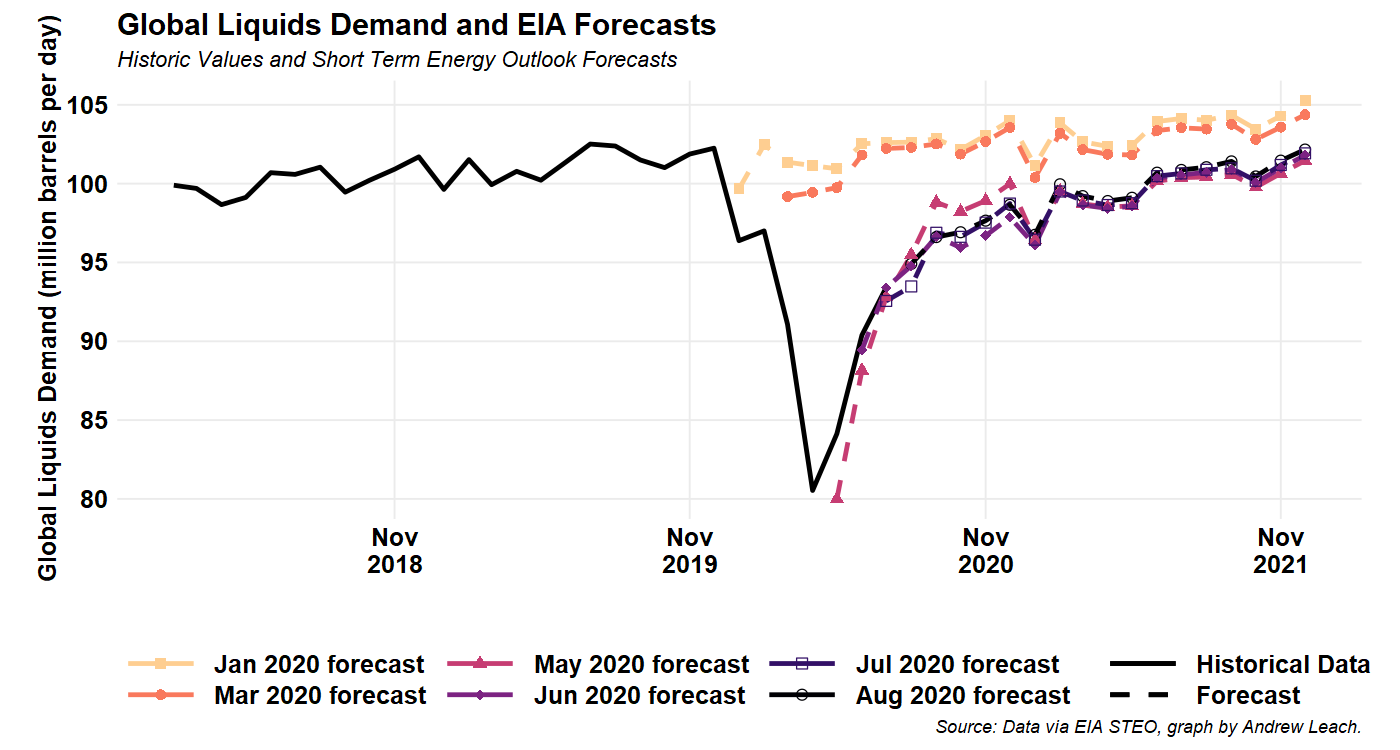
\includegraphics[width=0.85\textwidth]{week_1_problems_files/figure-latex/demand_new.png}
\end{enumerate}




\end{document}

